\documentclass[tikz, border=10pt]{standalone}
\usetikzlibrary{positioning, calc, backgrounds, shapes.geometric}

\begin{document}
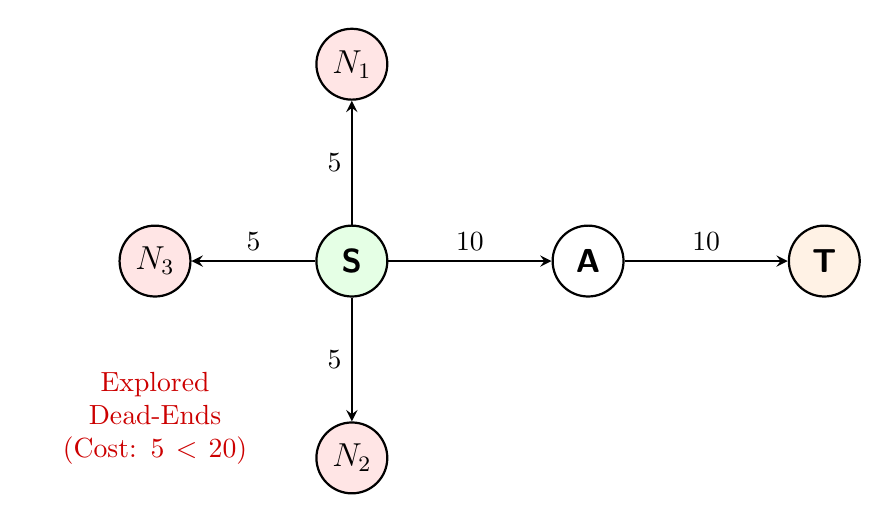
\begin{tikzpicture}[
    node distance=1.5cm and 2cm,
    vertex/.style={circle, draw, thick, minimum size=0.9cm, inner sep=1pt, font=\sffamily\large\bfseries},
    directed/.style={->, >=stealth, thick}
]
    % Main Path Nodes
    \node[vertex, fill=green!10] (S) at (0, 0) {S};
    \node[vertex] (A) at (3, 0) {A};
    \node[vertex, fill=orange!10] (T) at (6, 0) {T};
    
    % Dead-end Nodes (Wrong Direction)
    \node[vertex, fill=red!10] (N1) at (0, 2.5) {$N_1$};
    \node[vertex, fill=red!10] (N2) at (0, -2.5) {$N_2$};
    \node[vertex, fill=red!10] (N3) at (-2.5, 0) {$N_3$};

    % Edges for main path
    \draw[directed] (S) -- node[above] {10} (A);
    \draw[directed] (A) -- node[above] {10} (T);
    
    % Edges for dead-ends
    \draw[directed] (S) -- node[left] {5} (N1);
    \draw[directed] (S) -- node[left] {5} (N2);
    \draw[directed] (S) -- node[above] {5} (N3);
    
    % Annotations
    \node[red!80!black, align=center, text width=3cm] at (-2.5, -2) {Explored Dead-Ends\\(Cost: $ 5 < 20$)};
\end{tikzpicture}
\end{document}